\subsection{Modélisation mathématique}

  Nous avons choisi de représenter nos graphes comme une liste de sommets,
  chacun ayant une liste d'arêtes.

  En mémoire, cette structure est donc constituée d'une liste de pointeurs
  vers des sommets. Les sommets contenant une liste de pointeurs vers des
  arêtes. Chaque arête ayant un pointeur vers chaque sommet extrêmité.

  Dans la suite nous noterons $n$ le nombre de sommets du graphe.

\subsection{Problème du voyageur de commerce}

\subsubsection{Analyse mathématique}
    Le problème du voyageur de commerce consiste à chercher un chemin passant
    par tous les sommets du graphe, de longueur minimale.
    Ce problème peut s'illustrer par l'exemple d'une
    fraiseuse qui doit percer des trous dans une plaque le plus
    rapidement possible, ou encore par un car de touristes qui souhaiterait
    trouver l'itinéraire le plus rapide pour visiter un certain nombre de lieux.

    On peut modéliser ce problème par un graphe complet, dont les arêtes ont un
    coup qui correspond à la distance entre chaque point, on cherche alors le
    cycle hamiltonien de coût minimal. On sait qu'un tel cycle existe car le
    graphe est complet.

    Cependant trouver un tel cycle est un problème NP-difficile, et il n'existe
    donc pas d'algorithme efficace pour trouver ce cycle.
    En effet, la seule méthode exacte consisterait à tester toutes les chaines
    hamiltoniennes, et à prendre celle la plus courte, mais le nombre de chaines
    hamiltonniennes croît exponentiellement du nombre de sommets dans le graphe.

    Nous allons donc nous concentrer sur les méthodes approchées de résolution,
    qui peuvent donner de très bons résultats tout en étant rapides.
    Toutefois, le résultat n'est donc pas forcément le plus court.

  \subsubsection{Heuristiques}

    Les heuristiques vont nous permettre de construire un chemin le plus court
    possible, de manière rapide, avec le moins de calcul possible.
    Étant donné qu'on est confronté à énormément de possibilitées pendant
    la recherche, ils vont permettre d'orienter cette dernière, en faisant
    des choix les plus judicieux possibles sur les possibilitées a explorer.

    \paragraph{Exemple} Un heuristique simple consiste à partir d'un sommet au hasard du graphe et
    d'aller au sommet le plus proche sur lequel on n'est pas encore passé (puis
    à retourner au sommet de départ pour boucler le cycle). Cet algorithme est
    en $O(n)$ et donc rapide. Mais il n'offre cependant aucune garantie de
    résultat, il existe même des graphes pour lesquels il donne le pire cycle.

    Plus généralement, chercher parmi les $p$ sommets les plus proches s'avère
    être une solution relativement efficace, avec une complexité en $O(p^n)$
    (donc toujours exponentielle si $p \neq 1$).

    Une méthode purement basée sur cet heuristique donnerait~:

    \begin{lstlisting}
Entrée : g (Graphe complet)
Sortie : (coût, cycle) où cycle est un cycle hamiltonien construit selon la méthode du plus proche voisin et coût son coût associé sous forme de liste de points
coût = 0
cycle = ["un point de g au hasard"]

tant qu'il reste des points:
    # On ajoute au cycle le point suivant
    plus_proche = "point de g sur lequel on est pas encore passé le plus proche du dernier point du cycle"

    coût += "coût de plus_proche au dernier point du cycle"
    cycle = cycle :: plus_proche

# On ferme le cycle
coût += "coût du dernier au premier point de cycle"
cycle = cycle :: "premier point de chaine"

retourner (coût, cycle)
    \end{lstlisting}

  \subsubsection{Recherche locale}

    Les heuristiques nous donnant des solutions acceptables, choisies avec un
    minimum de «~bon sens~», il est ensuite possible de tenter d'améliorer
    ces solutions, via de la recherche locale.
    Partant d'une solution fournie, on va explorer les solutions voisines
    à cette dernière, afin de voire si on pourrait pas trouver des solutions
    encore meilleures parmi leur voisinage.

    \paragraph{Exemple} Un algorithme de recherche locale adapté au problème
    du voyageur de commerce est le 2-opt.
    Le principe du 2-opt consiste à tenter d'éliminer les «~boucles~» qui
    pourraient survenir dans le chemin, afin de le rendre plus court.

    Ainsi, partant du chemin suivant (qu'on obtendrait logiquement en suivant
    l'heuristique consistant à aller sur le sommet le plus près)~:

    \begin{center}
    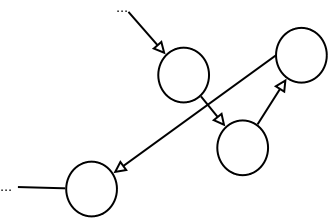
\includegraphics[width=0.3\textwidth]{graphes/2opt1.png}
    \end{center}

    On obtiendrait ceci, en éliminant le croisement~:

    \begin{center}
    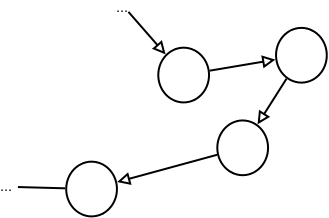
\includegraphics[width=0.3\textwidth]{graphes/2opt2.png}
    \end{center}

    L'algorithme pour le 2-opt est le suivant :
      \begin{lstlisting}
Entrée : un cycle hamiltonien (liste de sommets) et son coût
Sortie : un cycle hamiltonien et son coût inférieur ou égal au coup d'entrée

pour chaque couple de points (a, b) dans le cycle:
    nouveau_coût = coût
                     - "coût de a à son successeur dans le cycle"
                     - "coût de b à son successeur dans le cycle"
                     + "coût de a à b"
                     + "coût du successeur de a et au successeur de b dans le cycle"

    si nouveau_coût < coût:
        coût = nouveau_coût
        cycle = cycle crée en échangeant a et b dans cycle

retourner (coût, cycle)
      \end{lstlisting}

    Il est donc en $O(n^2)$ du nombre de sommets du cycle.

    L'application du 2-opt sur le chemin obtenu via un heuristique simple
    peut donner des résultats plus proches de la solution optimale qu'on
    pourrait le penser, et la combinaison des deux est donc une bonne méthode.

  \subsubsection{Métaheuristiques}

  Plutôt que d'utiliser un simple heuristique pour trouver une solution à priori plutôt
  bonne, puis d'y appliquer une recherche locale pour tenter de l'améliorer encore,
  il est possible d'utiliser des «~métaheuristiques~».
  Ces algorithmes vont avoir besoin d'heuristiques et de recherche locale, mais vont
  s'en servir en boucle, pour tenter sans cesse de trouver une solution meilleure.

  Ils vont partir explorer différentes parties de l'espace, souvent en guidant leur exploration
  grâce à l'heuristique, et en essayant de retomber sur des parties de l'espace les plus intéressantes
  possibles grâce aux algorithmes de recherche locale.

  Il existe énormément de métaheuristiques. En voici quelques uns :
  \begin{description}
  \item[Recherche locale itérée] méta-heuristique très simple consistant à utiliser un heuristique
                                 puis appliquer de la recherche locale pour améliorer son résultat.
                                 Ensuite, on perturbe légèrement ce résultat, on applique à nouveau
                                 une recherche locale et on recommence.
  \item[Recherche tabou] Amélioration de la recherche locale itérée, qui va utiliser une «~liste tabou~»
                         banissant toute recherche autour des zones de l'espace déjà explorées.
  \item[Recuit simulé] explore d'abord l'espace sans se restreindre aux parties donnant des solutions
                       efficaces, puis se restreint de plus en plus au voisinage des solutions les
                       plus efficaces. Converge donc vers les solutions les plus efficaces trouvées,
                       puis relâche les contraintes et explore autour de ces dernières, quitte à
                       trouver des solutions vraiment moins efficace. Recommence à se contraindre
                       aux plus efficaces, etc…
  \item[Algorithmes génétiques] imitent de la sélection naturelle, avec une population de solutions
                                qui évoluent en mutant et en s'échangeant leurs caractéristiques
                                entre elles. On peut même faire évoluer des populations séparément
                                avec les modèles en îles, pour avoir plusieurs populations très
                                différentes.
  \item[Colonies de fourmis] imitent la encore la nature en simulant des phéromones déposées par des
                             fourmis virtuelles, qui orientent la recherche au fil du temps.
  \item[...]
  \end{description}

  \subsubsection{Conclusion}

  Il est intéressant de constater que les heuristiques, méthodes de recherche locales,
  ainsi que les méta-heuristiques sont des choses extrêmement générales, utilisées
  pour résoudre énormément de problèmes demandant d'explorer un espace extrêmement grand.

  Elles ne sont donc pas propres au voyageur du commerce, même si on a vu comment, dans
  le cas précis du voyageur du commerce, on pouvait obtenir des résultats corrects en se
  passant de métaheuristiques. On pourrait donc améliorer ces résultats en en utilisant.
